\documentclass[UTF8]{ctexart}

\title{电子技术基础实验第十周实验报告}

\author{王磊\quad2022012972}

\date{\today}

\usepackage{geometry}
\geometry{a4paper,scale=0.8}

\usepackage{graphicx}
\usepackage{subfigure}
\usepackage{float}

\usepackage{amsmath}

\usepackage{listings}
\usepackage{xcolor}
\usepackage{framed}
\usepackage{placeins}
\lstdefinestyle{verilogStyle}{
    language=verilog,
    basicstyle=\ttfamily,
    keywordstyle=\color{blue},
    commentstyle=\color{green},
    stringstyle=\color{red},
    numbers=left,
    numberstyle=\tiny\color{gray},
    breaklines=true,
    showstringspaces=false,
    columns = fixed,
    basewidth = 0.5em,
    captionpos=b,
}
\newcommand{\subsubsubsection}[1]{\paragraph{#1}\mbox{}\\}
\setcounter{secnumdepth}{4} % how many sectioning levels to assign numbers to
\setcounter{tocdepth}{4} % how many sectioning levels to show in ToC
%设置段落间距
\setlength{\parskip}{0.5em}
%令小标题左对齐
\CTEXsetup[format={\Large\bfseries}]{section}
%首行不缩进
\setlength{\parindent}{0pt}
\begin{document}
\maketitle
%小标题
\section{task1\&task2}
由于task2是task1的延续,所以将两个任务放在一起说明。
\subsection{mif文件的生成}
为减少ROM的使用,我通过IP核生成了一个8位宽,768位深的ROM,将其分为三部分分别存储正弦波、三角波和方波。生成mif的matlab代码如图\ref{fig:matlab}所示。
\begin{figure}[!ht]
    \centering
    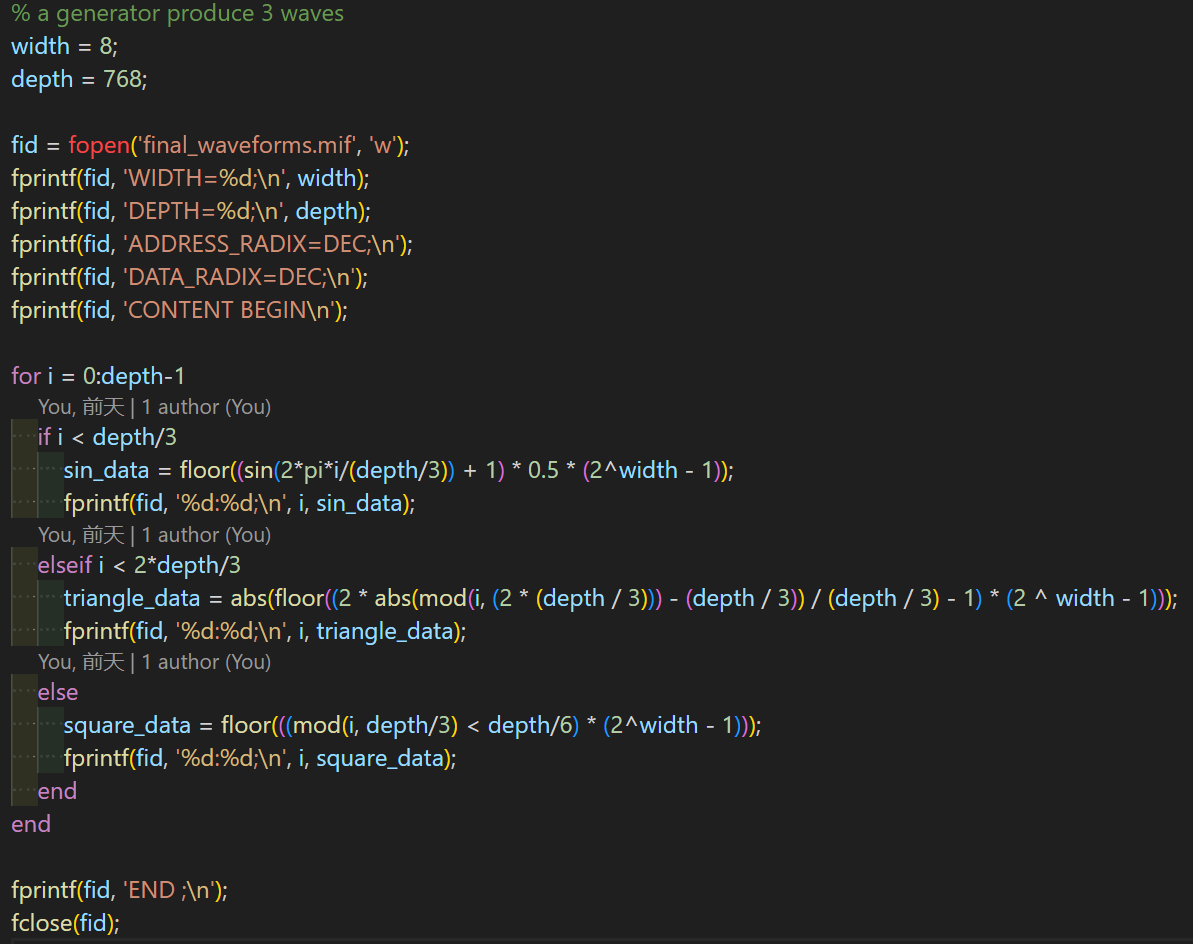
\includegraphics[width=0.8\textwidth]{matlab.png}
    \caption{matlab代码}
    \label{fig:matlab}
\end{figure}

\subsection{地址生成模块}
地址生成模块的代码如下:
\begin{framed}
    \begin{lstlisting}[style=verilogStyle]
module addr_tx_en2 (
    input clk,
    input clk_origin,
    input rst,
    input [2:0] switch,
    output reg [9:0] addr,
    output reg tx_en
);

    reg [9:0] addr_temp;
    always @(posedge clk, posedge rst) begin
        if (rst) begin
            addr_temp <= 10'd0;
        end else begin
            if (addr_temp == 10'd255) begin
                addr_temp <= 10'd0;
            end else begin
                addr_temp <= addr_temp + 1'b1;
            end
        end
    end

    always @(posedge clk, posedge rst) begin
        if (rst) begin
            addr <= 10'd0;
        end else begin
            if (switch[0]) begin
                addr <= addr_temp;
            end else if (switch[1]) begin
                addr <= addr_temp + 10'd256;
            end else if (switch[2]) begin
                addr <= addr_temp + 10'd512;
            end else begin
                addr <= 10'd0;
            end
        end
    end

    reg pulse1, pulse2, pulse3;
    wire clk_posedge;
    always @(posedge clk_origin, posedge rst) begin
        if (rst) begin
            pulse1 <= 1'b0;
            pulse2 <= 1'b0;
            pulse3 <= 1'b0;
        end else begin
            pulse1 <= clk;
            pulse2 <= pulse1;
            pulse3 <= pulse2;
        end
    end
    assign clk_posedge = pulse2 & ~pulse3;

    always @(posedge clk_origin, posedge rst) begin
        if (rst) begin
            tx_en <= 1'b0;
        end else begin
            if (clk_posedge) begin
                tx_en <= 1'b1;
            end else begin
                tx_en <= 1'b0;
            end
        end
    end


endmodule
    \end{lstlisting}
\end{framed}
其中,根据switch的值,addr\_temp会分别加上0、256、512,从而实现地址的切换。tx\_en则是通过检测分频时钟的上升沿在每次地址切换时产生一个脉冲,用于触发输出模块。

\subsection{顶层模块}
顶层模块的代码如下:
\begin{framed}
    \begin{lstlisting}[style=verilogStyle]
// Purpose: Top level module for UART transmit.
`include "addr_tx_en2.v"
`include "uart_transmit2.v"
`include "uart2_fre_div.v"
`include "three_waves_rom.v"
module uart2_top(
    input clk,
    input rst,
    input [2:0] switch,
    output  sci_tx
);

wire clk_div_addr;
uart2_fre_fiv uut1(
    .clk(clk),
    .rst(rst),
    .clk_div_addr(clk_div_addr)
);

wire [9:0] addr;
wire tx_en;
addr_tx_en2 uut2(
    .clk_origin(clk),
    .clk(clk_div_addr),
    .rst(rst),
    .switch(switch),
    .addr(addr),
    .tx_en(tx_en)
);

wire [9:0]data_temp;
three_waves_rom uut3(
    .address(addr),
    .clock(clk),
    .q(data_temp)
);

uart_transmit2 uut4(
    .clk(clk),
    .rst(rst),
    .tx_en(tx_en),
    .rx_d(data_temp),
    .sci_tx(sci_tx)
);



endmodule
    \end{lstlisting}
\end{framed}
RTL图如图\ref{fig:rtl}所示。
\begin{figure}[!ht]
    \centering
    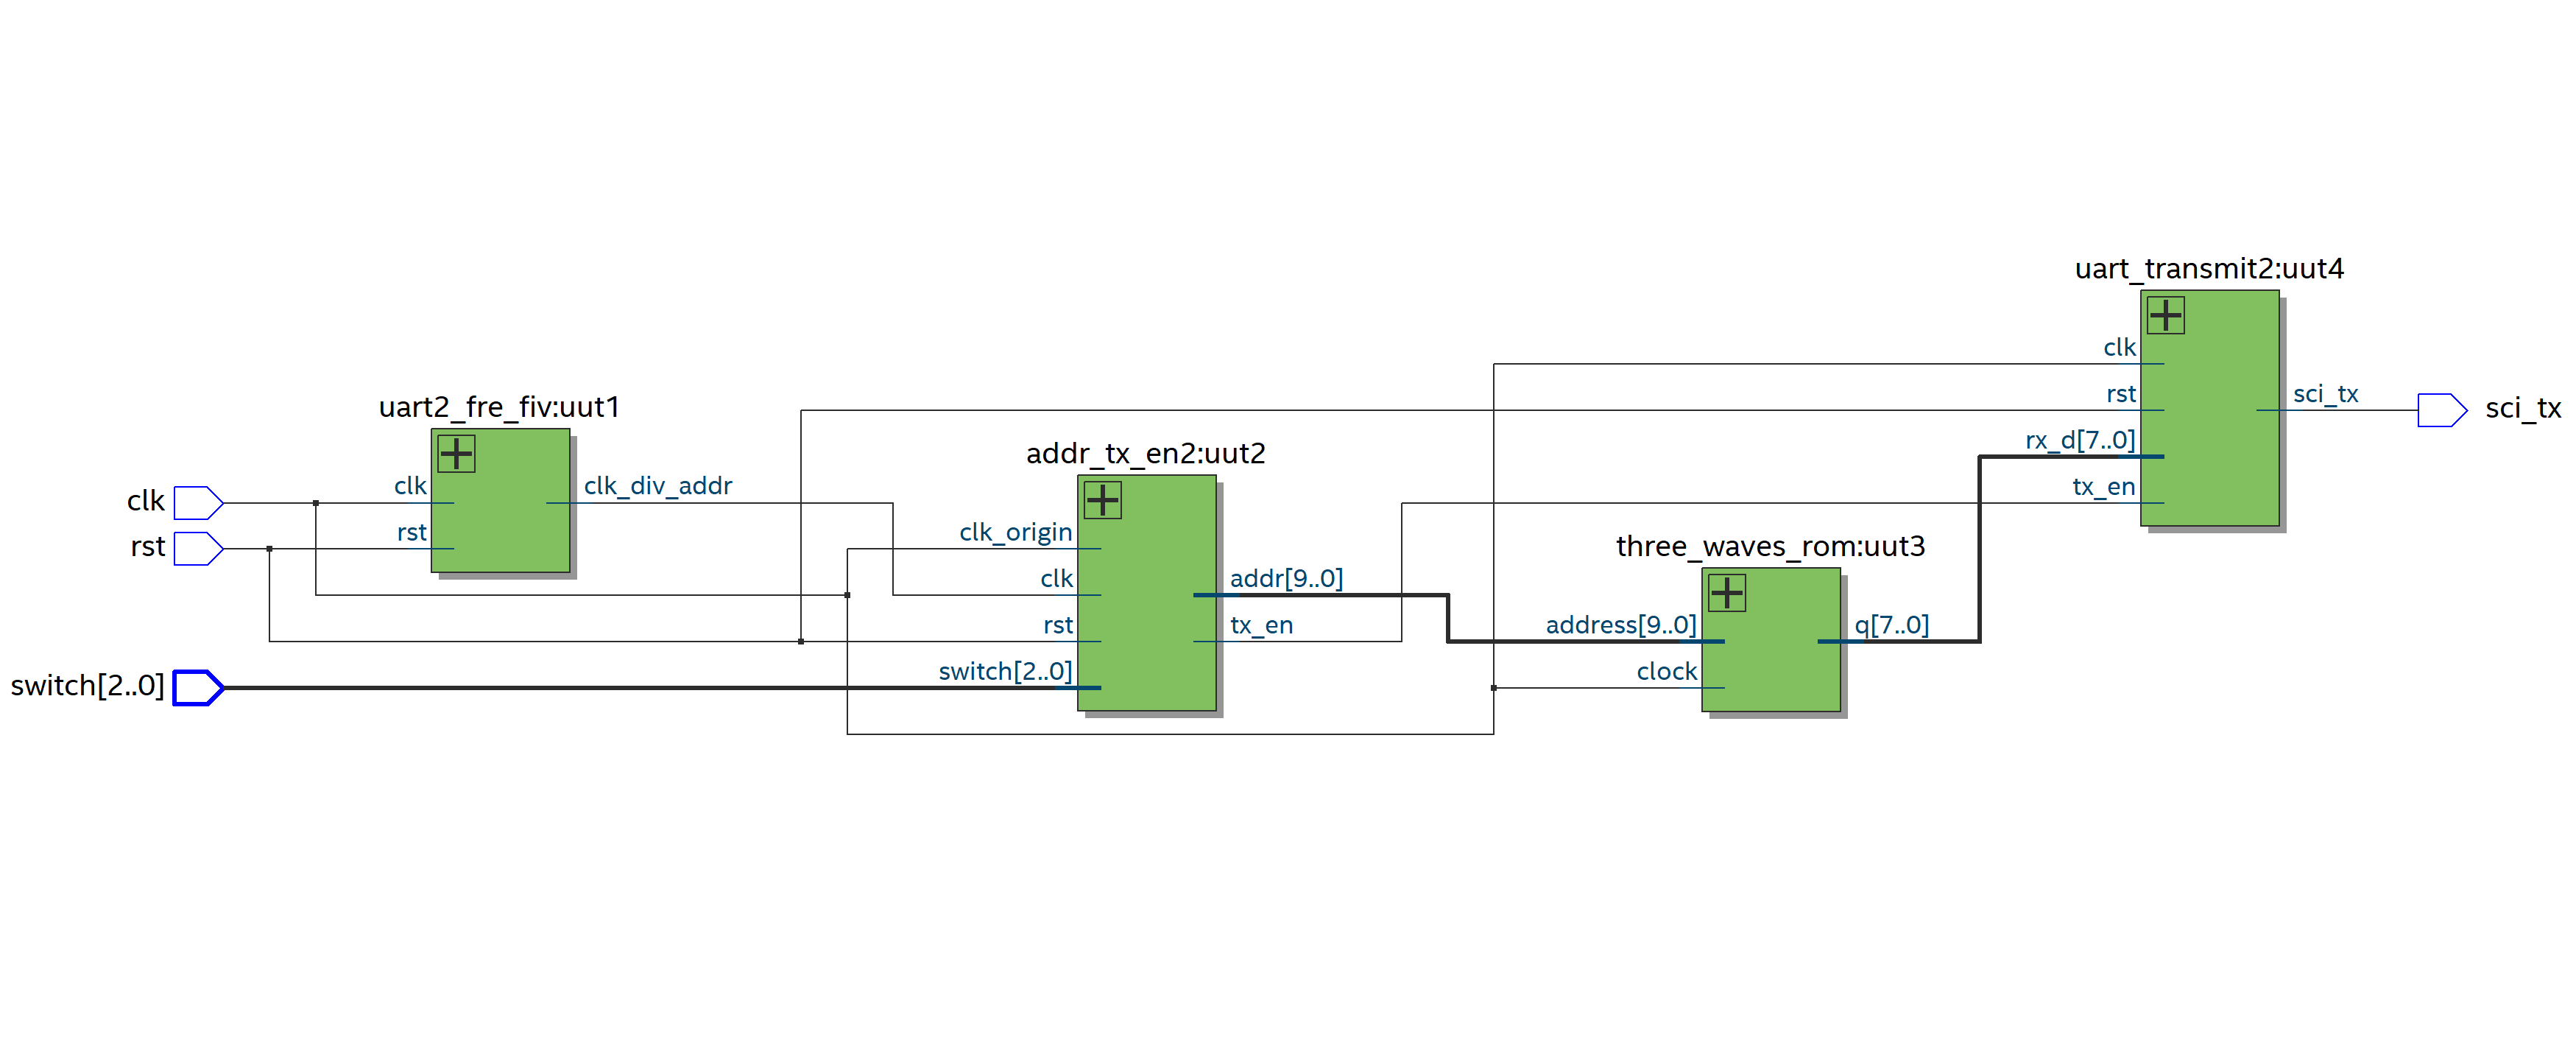
\includegraphics[width=0.8\textwidth]{rtl1.png}
    \caption{RTL图}
    \label{fig:rtl}
\end{figure}
\subsection{输出结果}
\FloatBarrier
输出结果如图\ref{fig:sine}、\ref{fig:triangle}、\ref{fig:square}所示。三个波形的频率均为50Hz,符合task1的要求。
\begin{figure}[!ht]
    \centering
    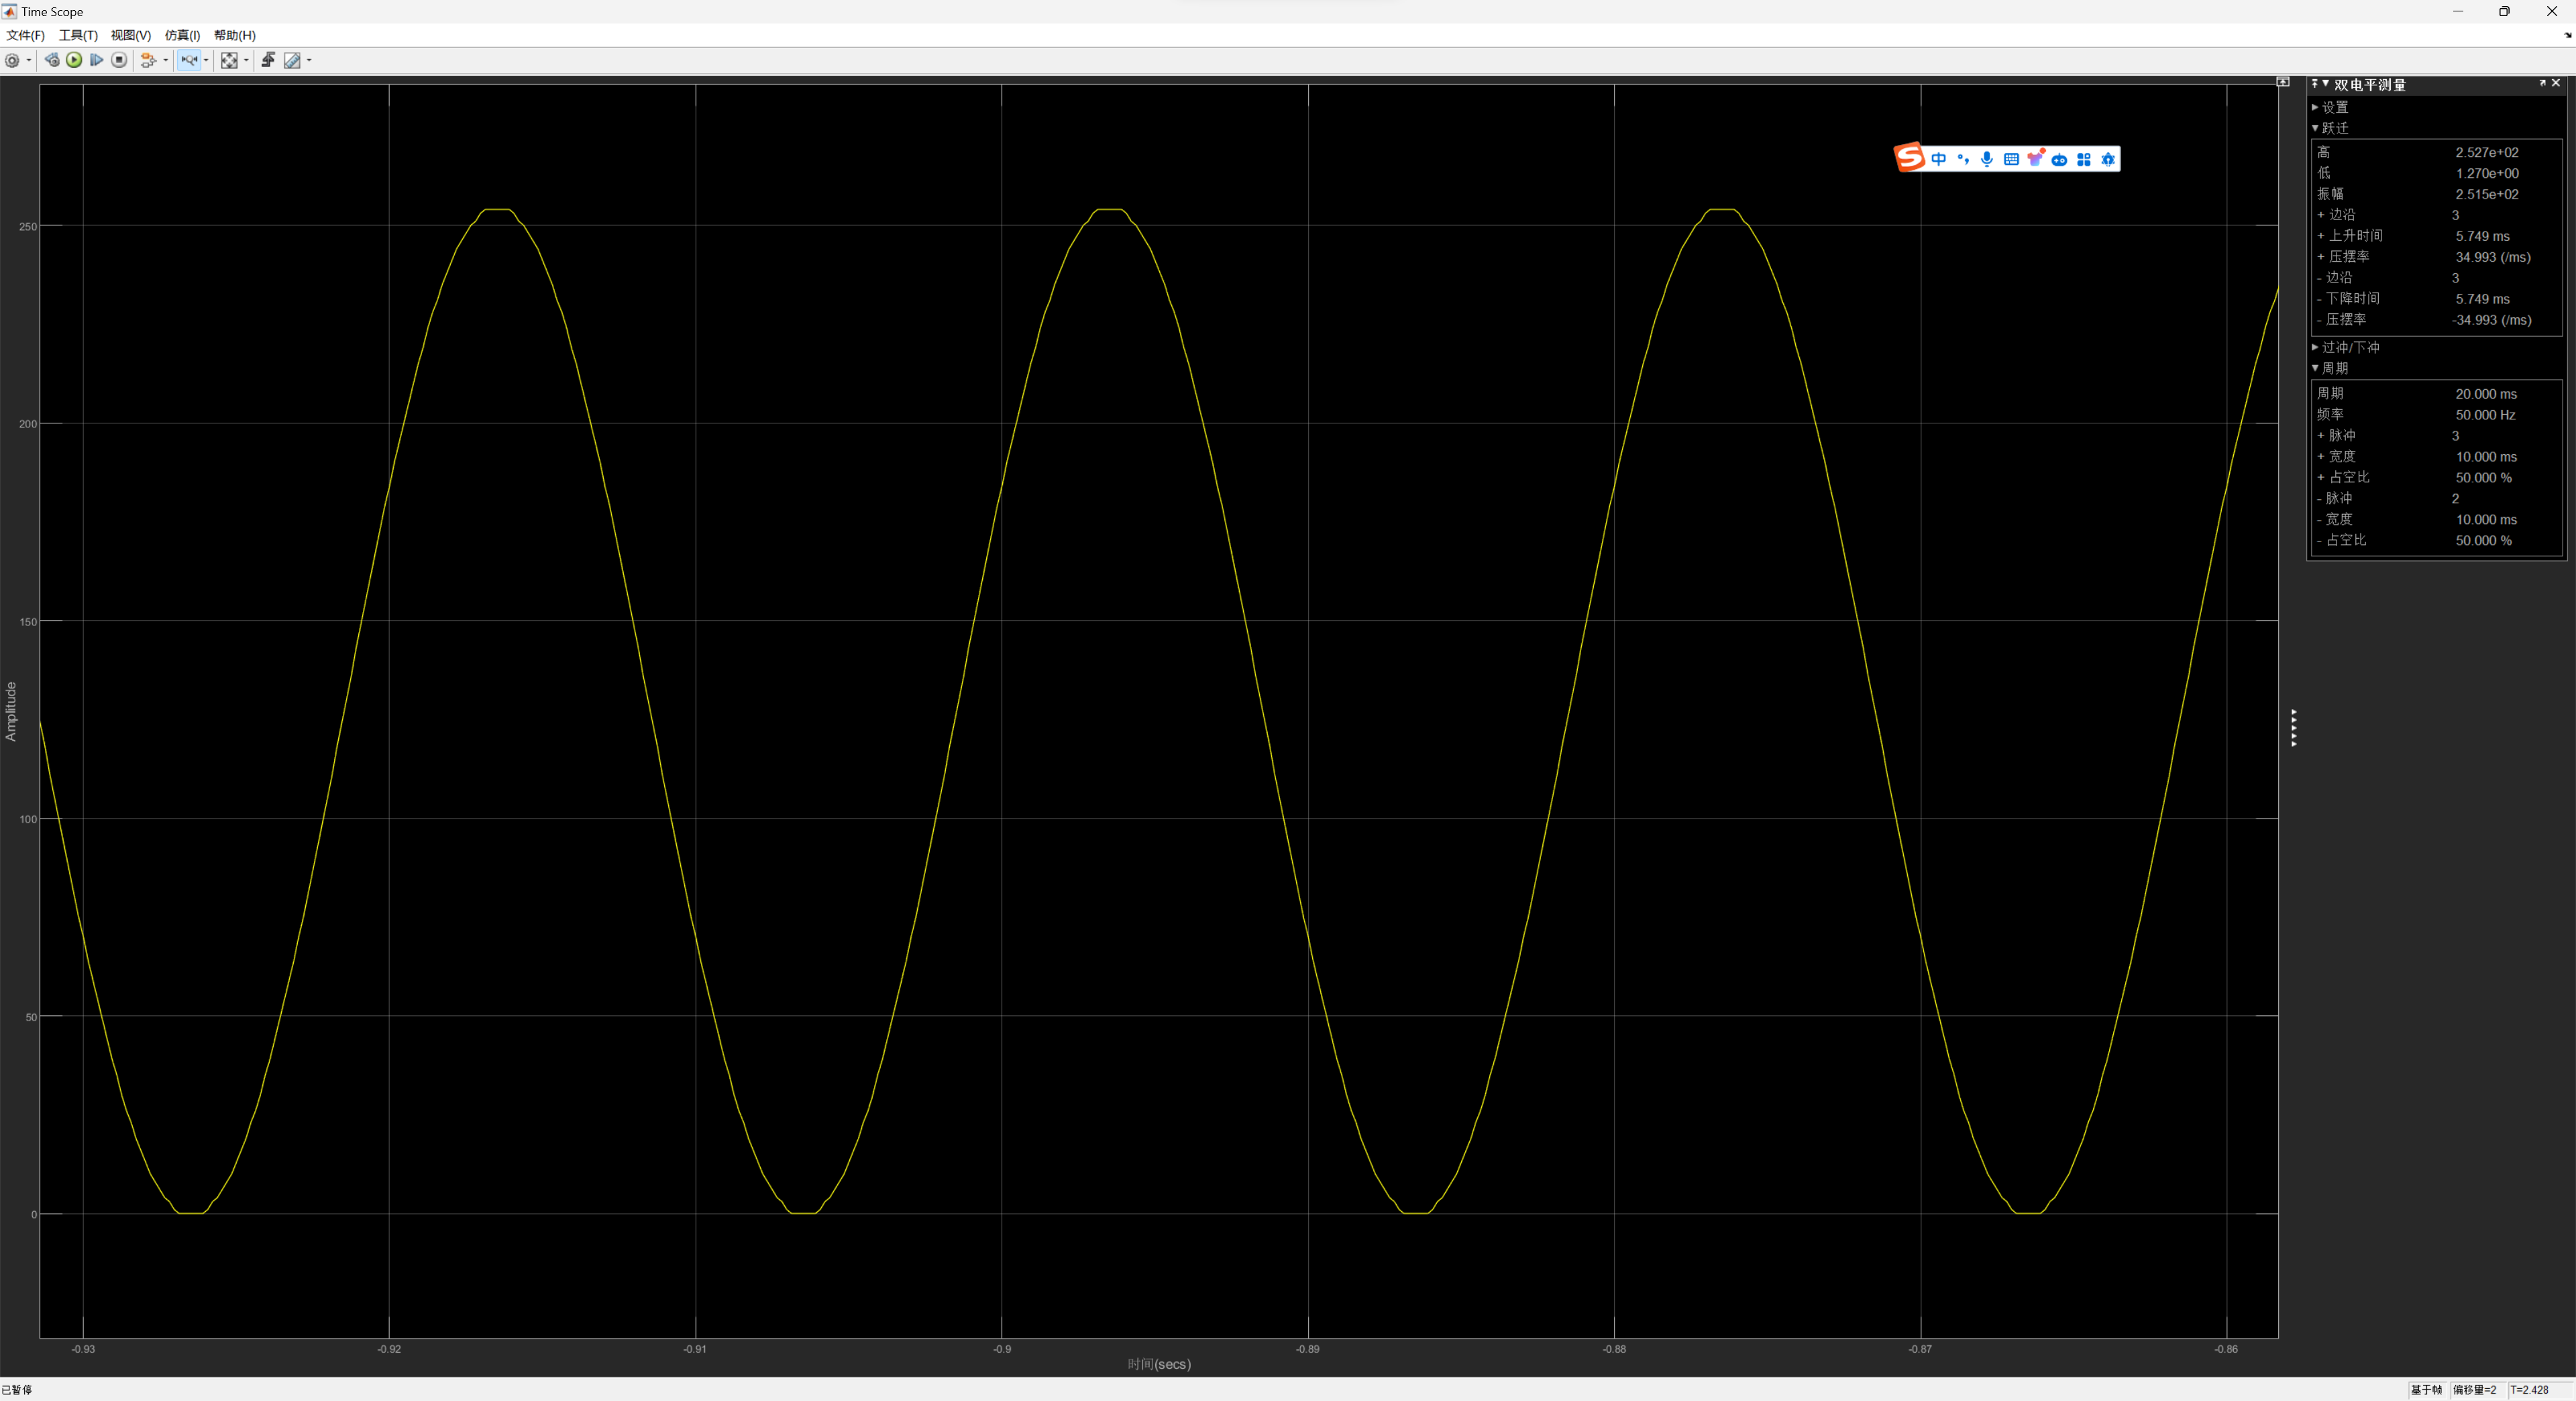
\includegraphics[width=0.8\textwidth]{sine.png}
    \caption{正弦波}
    \label{fig:sine}
\end{figure}
\begin{figure}[!ht]
    \centering
    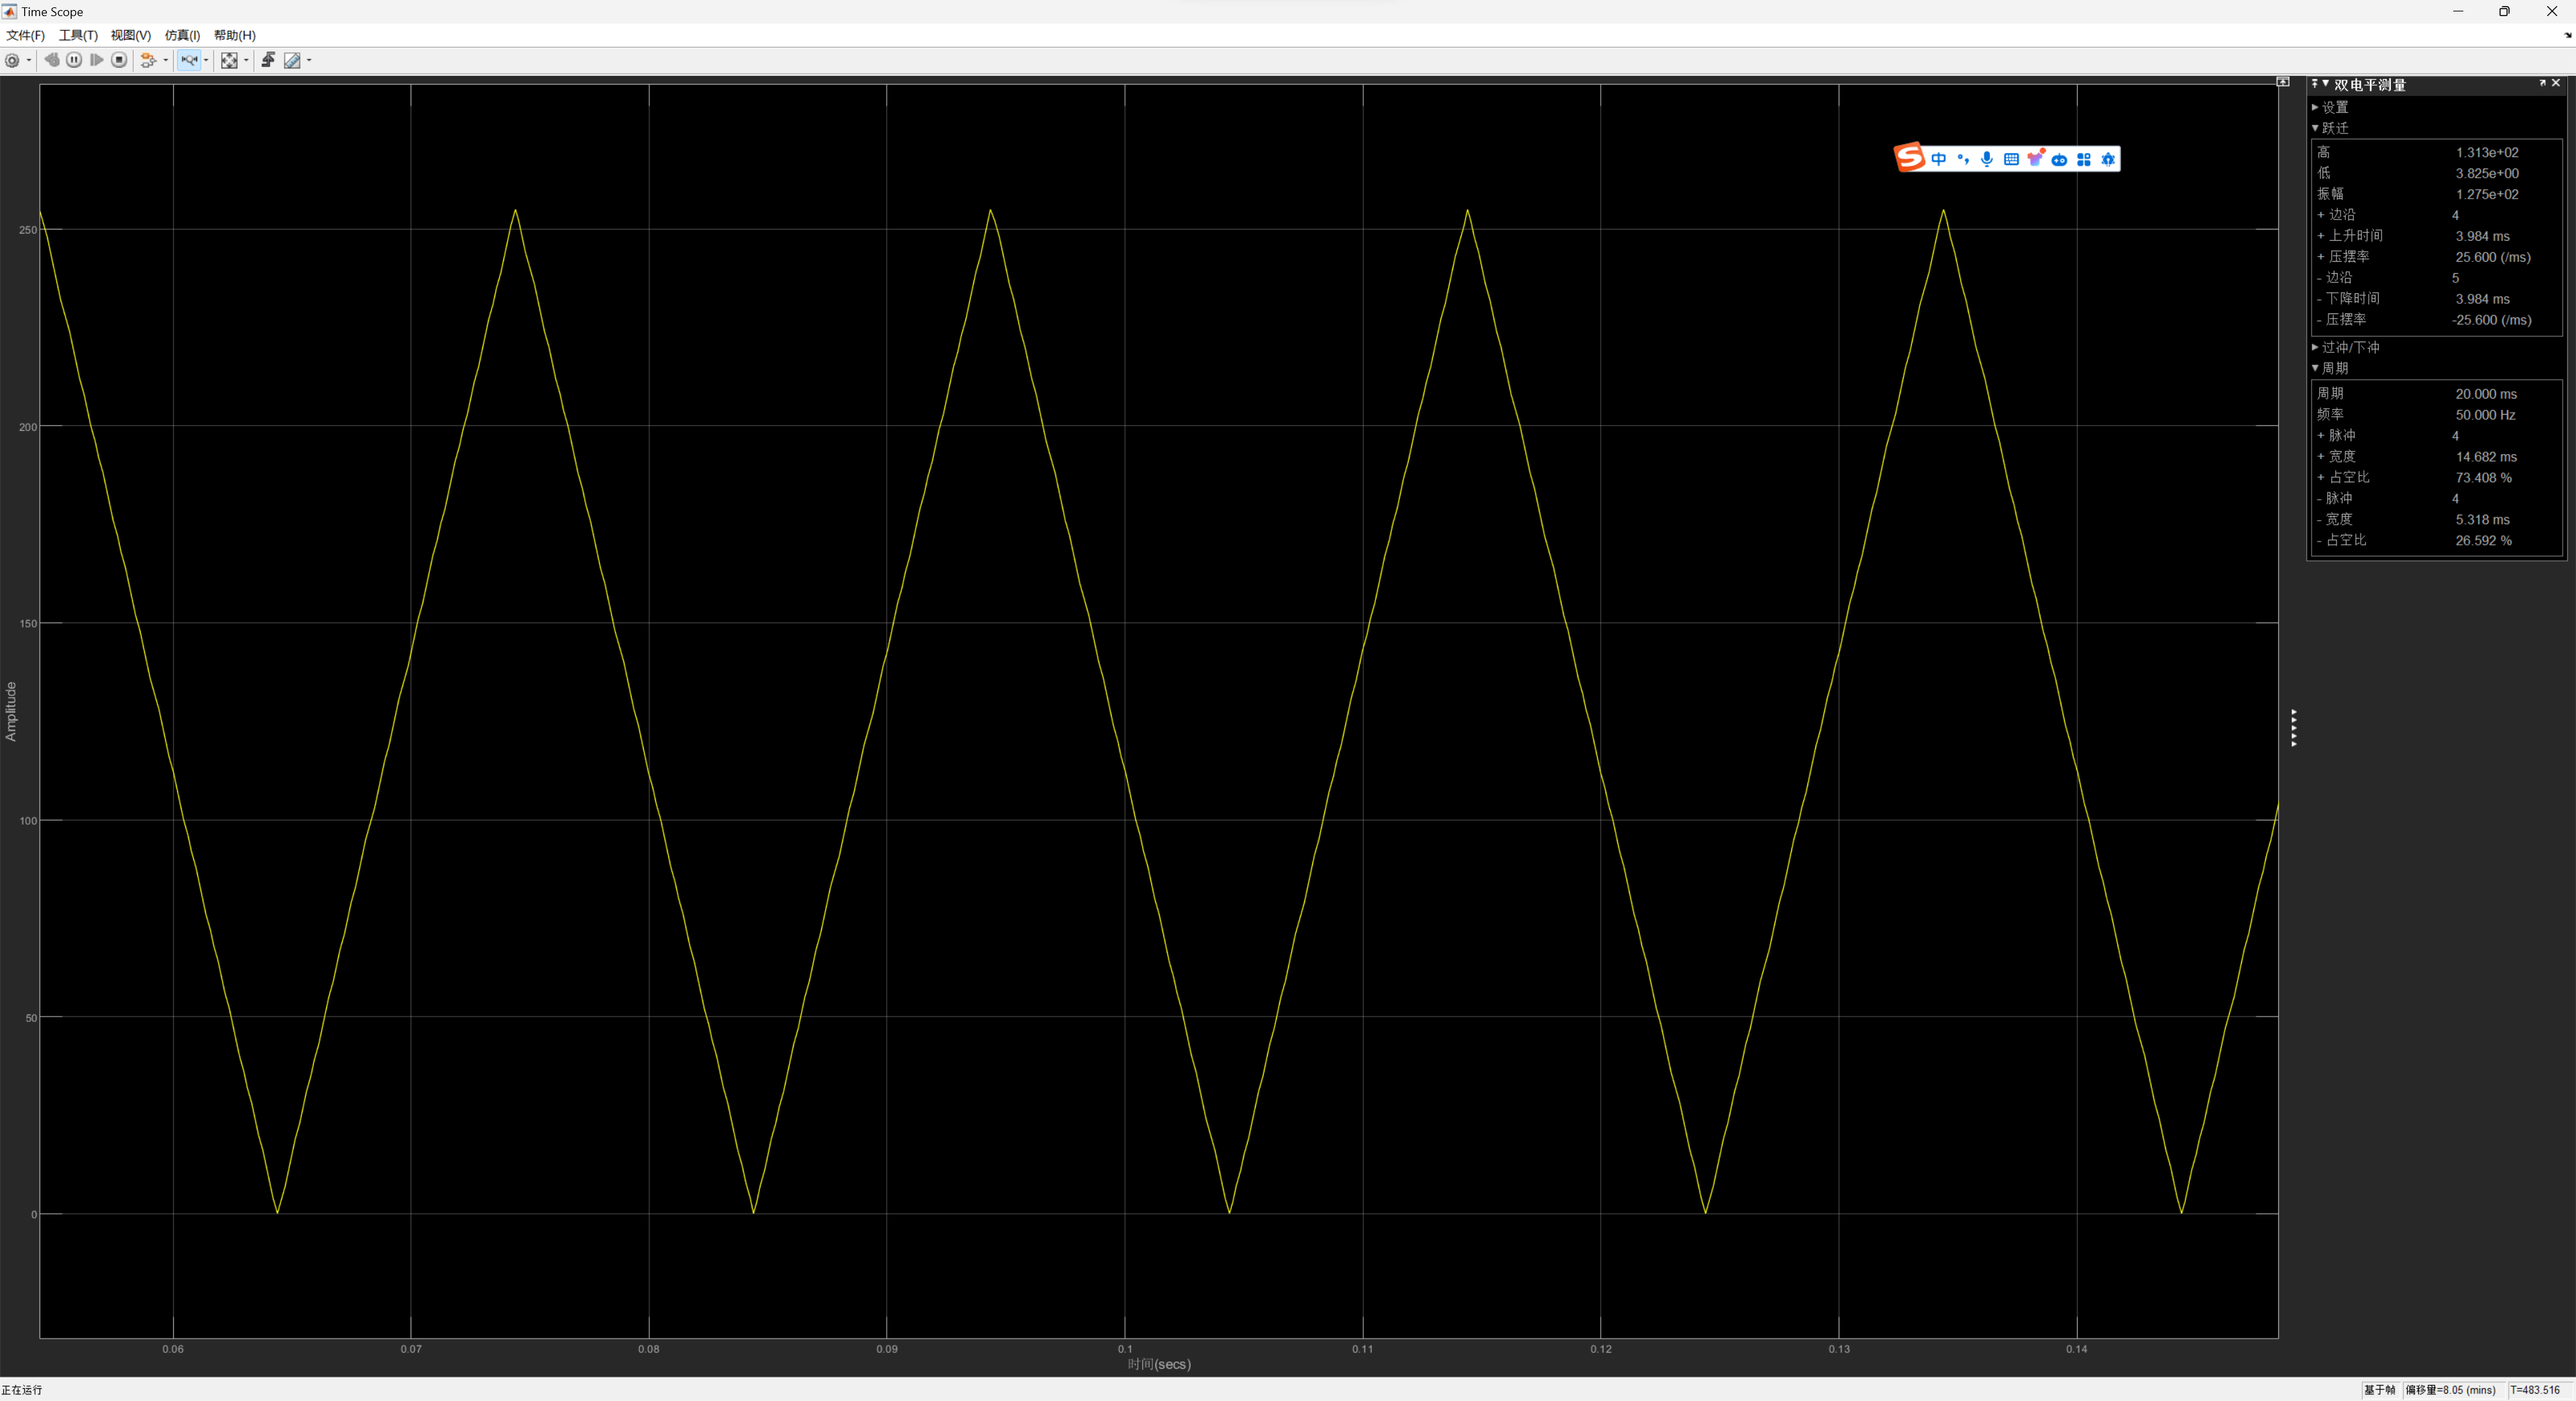
\includegraphics[width=0.8\textwidth]{triangle.png}
    \caption{三角波}
    \label{fig:triangle}
\end{figure}
\begin{figure}[!ht]
    \centering
    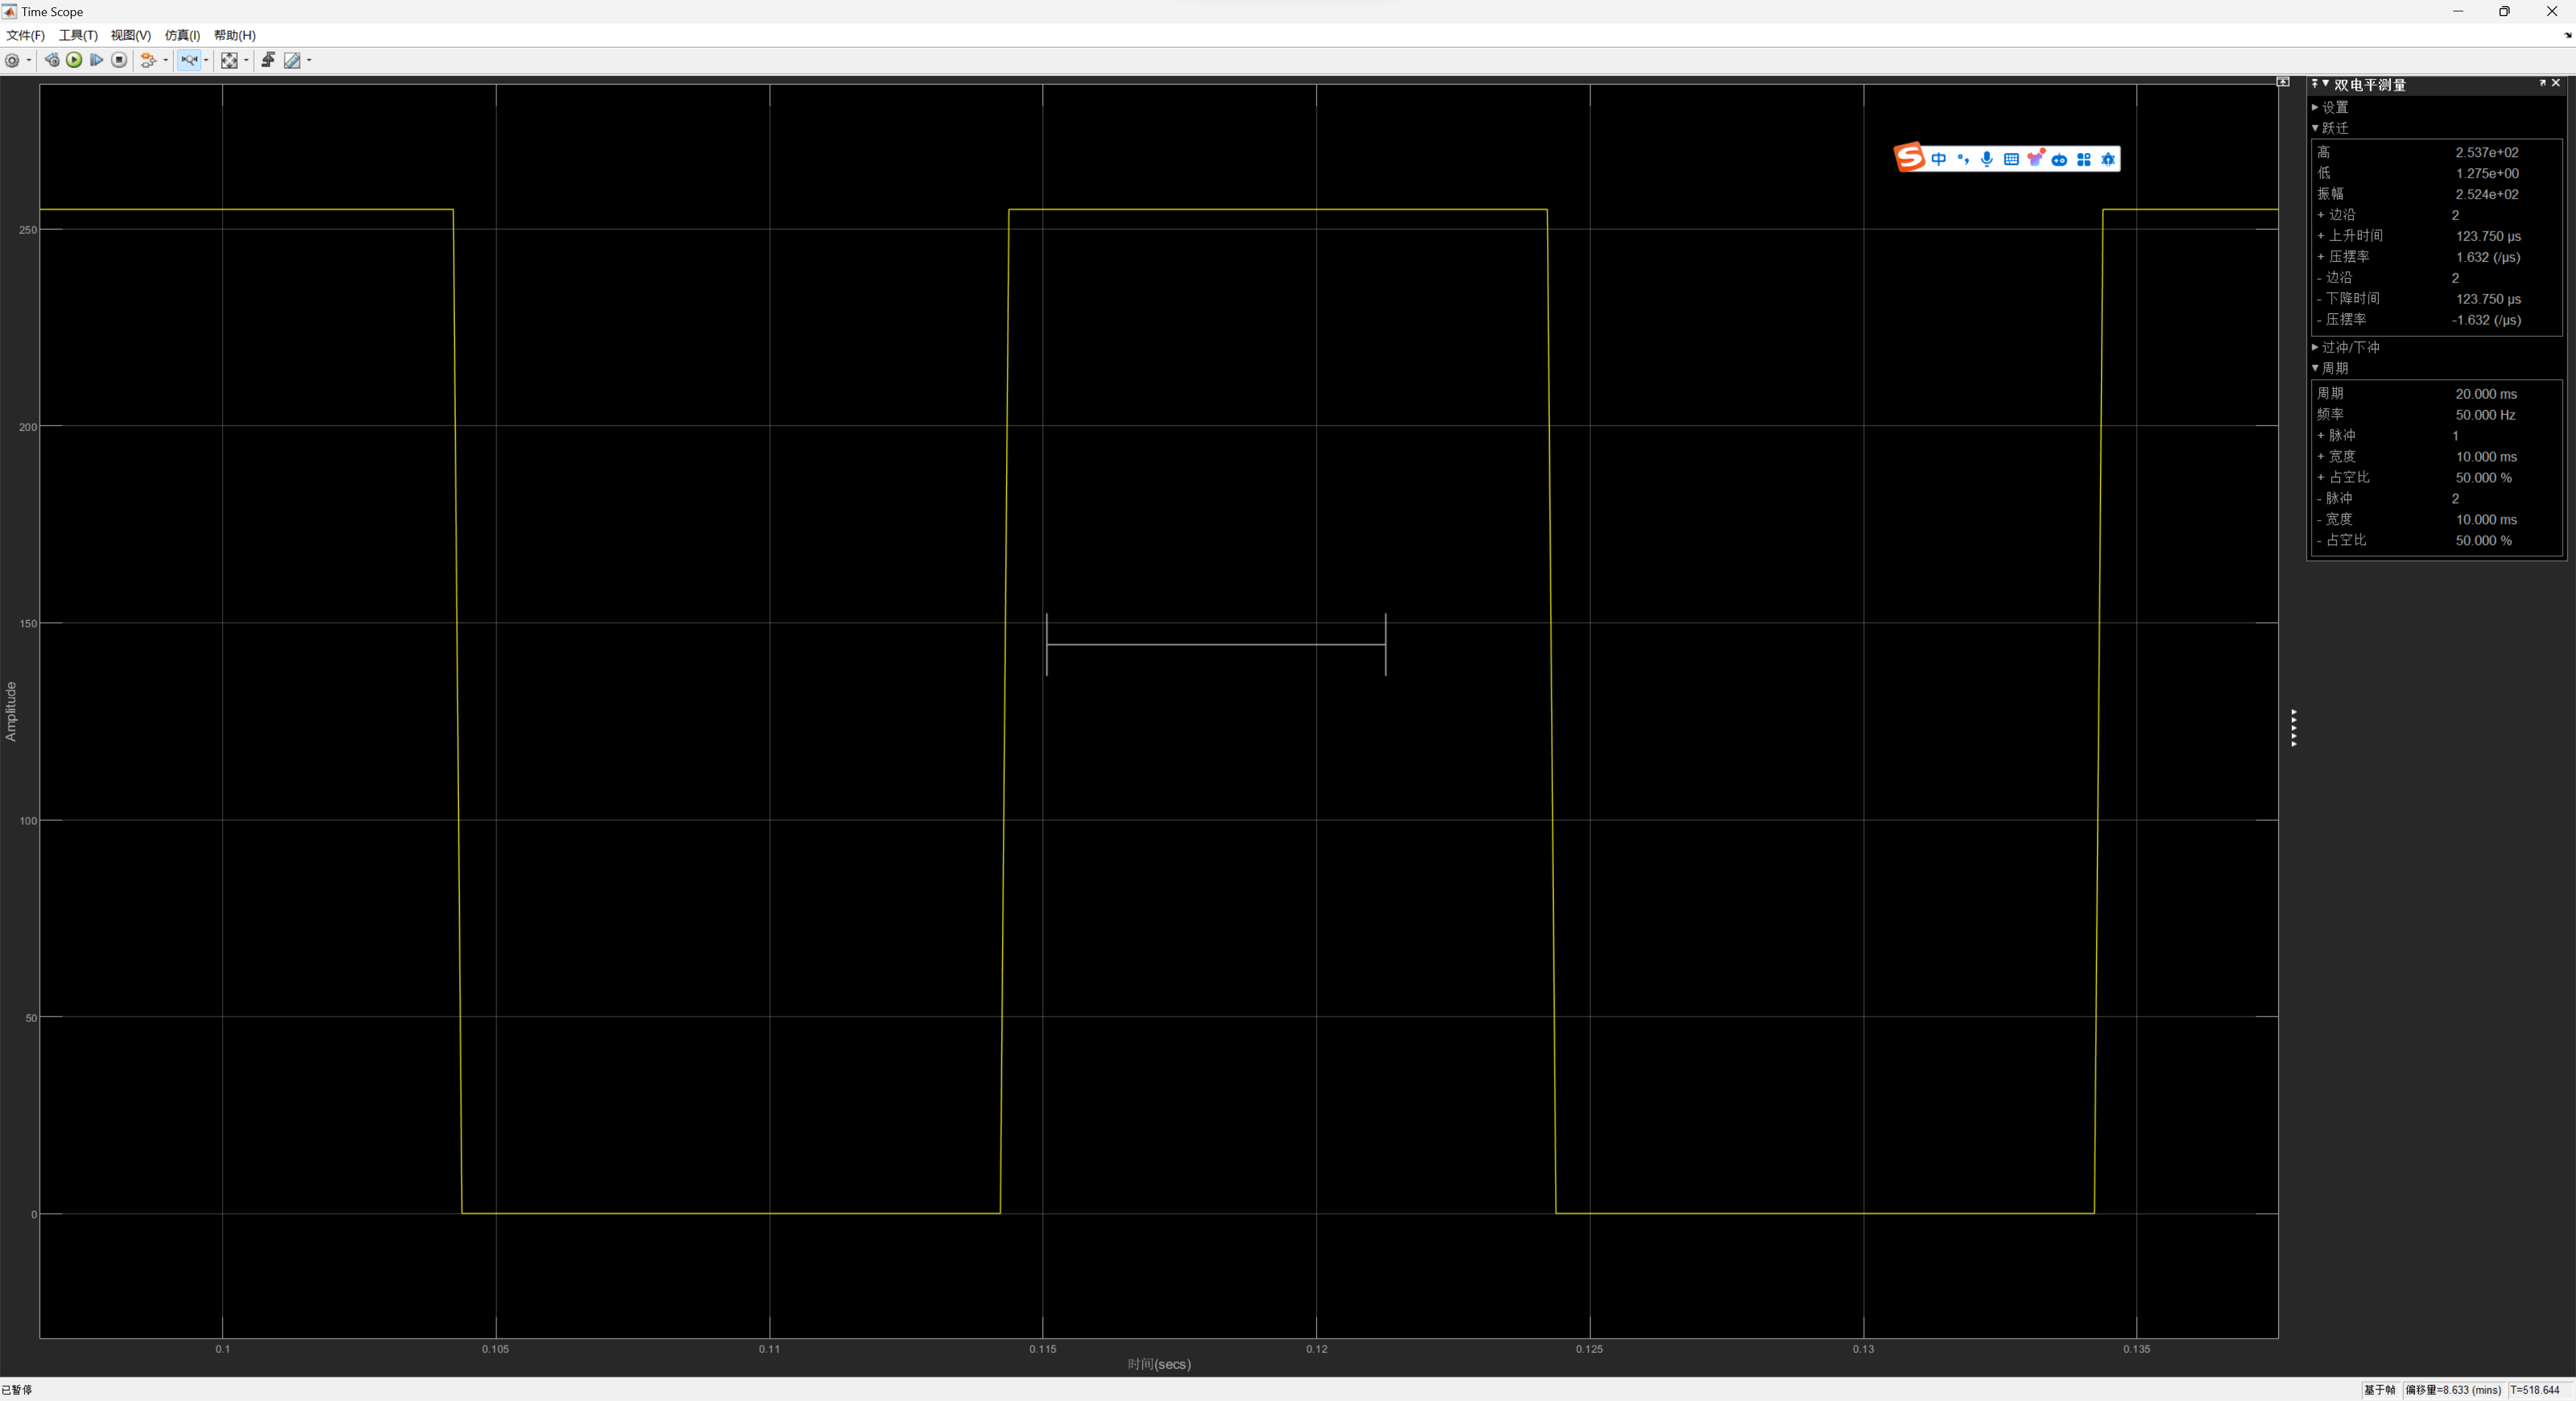
\includegraphics[width=0.8\textwidth]{square.png}
    \caption{方波}
    \label{fig:square}
\end{figure}
\FloatBarrier
\section{task3}
task3中FPGA计算及显示的部分与上周任务相似,只需要更改数据转换部分。数码管部分不加赘述。
\subsection{串口接收模块}
串口接收模块的代码如下:
\begin{framed}
    \begin{lstlisting}[style=verilogStyle]
module uart_receive #(
    parameter BAUD_RATE = 'd115200,
    parameter CLK_FREQ  = 25000000
) (
    input clk,
    input rst,
    input rx,
    output reg [7:0] data,
    output reg ready
);

    //localparam define
    localparam BAUD_CNT_MAX = CLK_FREQ / BAUD_RATE;

    //reg define
    reg rx_reg1;
    reg rx_reg2;
    reg rx_reg3;  //for pulse
    reg start_nedge;
    reg work_en;
    reg [12:0] baud_cnt;
    reg bit_flag;
    reg [3:0] bit_cnt;
    reg [7:0] rx_data;
    reg rx_flag;

    always @(posedge clk, posedge rst) begin
        if (rst) begin
            rx_reg1 <= 1'b1;
            rx_reg2 <= 1'b1;
            rx_reg3 <= 1'b1;
        end else begin
            rx_reg1 <= rx;
            rx_reg2 <= rx_reg1;
            rx_reg3 <= rx_reg2;
        end
    end

    always @(posedge clk, posedge rst) begin
        if (rst) begin
            start_nedge <= 1'b0;
        end else if ((~rx_reg2) && rx_reg3) begin
            start_nedge <= 1'b1;
        end else begin
            start_nedge <= 1'b0;
        end
    end

    always @(posedge clk, posedge rst) begin
        if (rst) begin
            work_en <= 1'b0;
        end else if (start_nedge) begin
            work_en <= 1'b1;
        end else if ((bit_cnt == 4'd8) && (bit_flag == 1'b1)) begin
            work_en <= 1'b0;
        end
    end

    always @(posedge clk, posedge rst) begin
        if (rst) begin
            baud_cnt <= 13'd0;
        end else if ((baud_cnt == BAUD_CNT_MAX - 1) || (work_en == 1'b0)) begin
            baud_cnt <= 13'd0;
        end else if (work_en) begin
            baud_cnt <= baud_cnt + 1'b1;
        end
    end

    always @(posedge clk, posedge rst) begin
        if (rst) begin
            bit_flag <= 1'b0;
        end else if (baud_cnt == BAUD_CNT_MAX / 2 - 1) begin
            bit_flag <= 1'b1;
        end else begin
            bit_flag <= 1'b0;
        end
    end

    always @(posedge clk, posedge rst) begin
        if (rst) begin
            bit_cnt <= 4'd0;
        end else if ((bit_cnt == 4'd8) && (bit_flag == 1'b1)) begin
            bit_cnt <= 4'd0;
        end else if (bit_flag == 1'b1) begin
            bit_cnt <= bit_cnt + 1'b1;
        end
    end

    always @(posedge clk, posedge rst) begin
        if (rst) begin
            rx_data <= 8'd0;
        end else if ((bit_cnt >= 4'd1) && (bit_cnt <= 4'd8) && (bit_flag == 1'b1)) begin
            rx_data <= {rx_reg3, rx_data[7:1]};
        end
    end

    always @(posedge clk, posedge rst) begin
        if (rst) begin
            rx_flag <= 1'b0;
        end else if ((bit_cnt == 4'd8) && (bit_flag == 1'b1)) begin
            rx_flag <= 1'b1;
        end else begin
            rx_flag <= 1'b0;
        end
    end

    always @(posedge clk, posedge rst) begin
        if (rst) begin
            data <= 8'd0;
        end else if (rx_flag) begin
            data <= rx_data;
        end
    end

    always @(posedge clk, posedge rst) begin
        if (rst) begin
            ready <= 1'b0;
        end else begin
            ready <= rx_flag;
        end
    end
endmodule
    \end{lstlisting}
\end{framed}
主要实现了如下核心功能:
\begin{itemize}
    \item 通过三个reg将rx打慢两拍,以消除亚稳态。
    \item 通过计数器实现指定波特率。
    \item 通过计数器实现中点读取数据,保证数据的稳定性。
    \item 在8位数据读取完毕后,将数据存入data中,同时将ready置1。
\end{itemize}

\subsection{通讯协议指定}
虽然任务要求使用十六进制发送并用数字指代运算符,但是我认为这种形式不是十分优雅,所以我将通讯协议改为了如下形式:\textbf{前数+运算符+后数+=}。其中+-=均有对应的ascll码,可以直接输入。而与、或和比较分别用A、O、C表示。这样的好处是串口输入较为直观,例如输入\textbf{1+2=}即可得到3。同时,这样的协议也可以很方便地扩展到更多的运算符上。
\subsection{数据转换模块}
数据转换模块的代码如下:
\begin{framed}
    \begin{lstlisting}[style=verilogStyle]
//process the origin input to a simple one
    reg [3:0] input_type;
    parameter NUMBER = 4'b0001;
    parameter OPERATOR = 4'b0010;
    parameter EQUAL = 4'b0100;
    parameter RESET = 4'b1000;
    reg [4:0] input_temp;
    reg input_flag;

    always @(posedge clk, posedge rst) begin
        if (rst) begin
            input_type <= 3'b000;
            input_temp <= 5'b00000;
            input_flag <= 1'b0;
        end else if (ready) begin
            case (rx_data)
                8'd48: begin
                    input_type <= NUMBER;
                    input_temp <= 5'b00000;
                end
                8'd49: begin
                    input_type <= NUMBER;
                    input_temp <= 5'b00001;
                end
                8'd50: begin
                    input_type <= NUMBER;
                    input_temp <= 5'b00010;
                end
                8'd51: begin
                    input_type <= NUMBER;
                    input_temp <= 5'b00011;
                end
                8'd52: begin
                    input_type <= NUMBER;
                    input_temp <= 5'b00100;
                end
                8'd53: begin
                    input_type <= NUMBER;
                    input_temp <= 5'b00101;
                end
                8'd54: begin
                    input_type <= NUMBER;
                    input_temp <= 5'b00110;
                end
                8'd55: begin
                    input_type <= NUMBER;
                    input_temp <= 5'b00111;
                end
                8'd56: begin
                    input_type <= NUMBER;
                    input_temp <= 5'b01000;
                end
                8'd57: begin
                    input_type <= NUMBER;
                    input_temp <= 5'b01001;
                end
                8'd43: begin
                    input_type <= OPERATOR;
                    input_temp <= ADD_OPERATOR;
                end
                8'd45: begin
                    input_type <= OPERATOR;
                    input_temp <= SUB_OPERATOR;
                end
                8'd65: begin
                    input_type <= OPERATOR;
                    input_temp <= AND_OPERATOR;
                end
                8'd79: begin
                    input_type <= OPERATOR;
                    input_temp <= OR_OPERATOR;
                end
                8'd67: begin
                    input_type <= OPERATOR;
                    input_temp <= COMPARE_OPERATOR;
                end
                8'd61: begin
                    input_type <= EQUAL;
                    input_temp <= 5'b00000;
                end
                8'd82: begin
                    input_type <= RESET;
                    input_temp <= 5'b00000;
                end
                default: begin
                    input_type <= 3'b000;
                    input_temp <= 5'b00000;
                    input_flag <= 1'b0;
                end
            endcase
        end else begin
            input_type <= 3'b000;
            input_temp <= 5'b00000;
            input_flag <= 1'b0;
        end
    end
    \end{lstlisting}
\end{framed}
以上代码将串口传入的字符处理为了上周所完成的计算器所需要的格式。其中,input\_type用于指示当前输入的类型,input\_temp则是处理后的数据。input\_flag用于指示是否有新的输入。
计算过程中还使用了mealy状态机,其示意图如图\ref{fig:mealy}所示。
\begin{figure}[!ht]
    \centering
    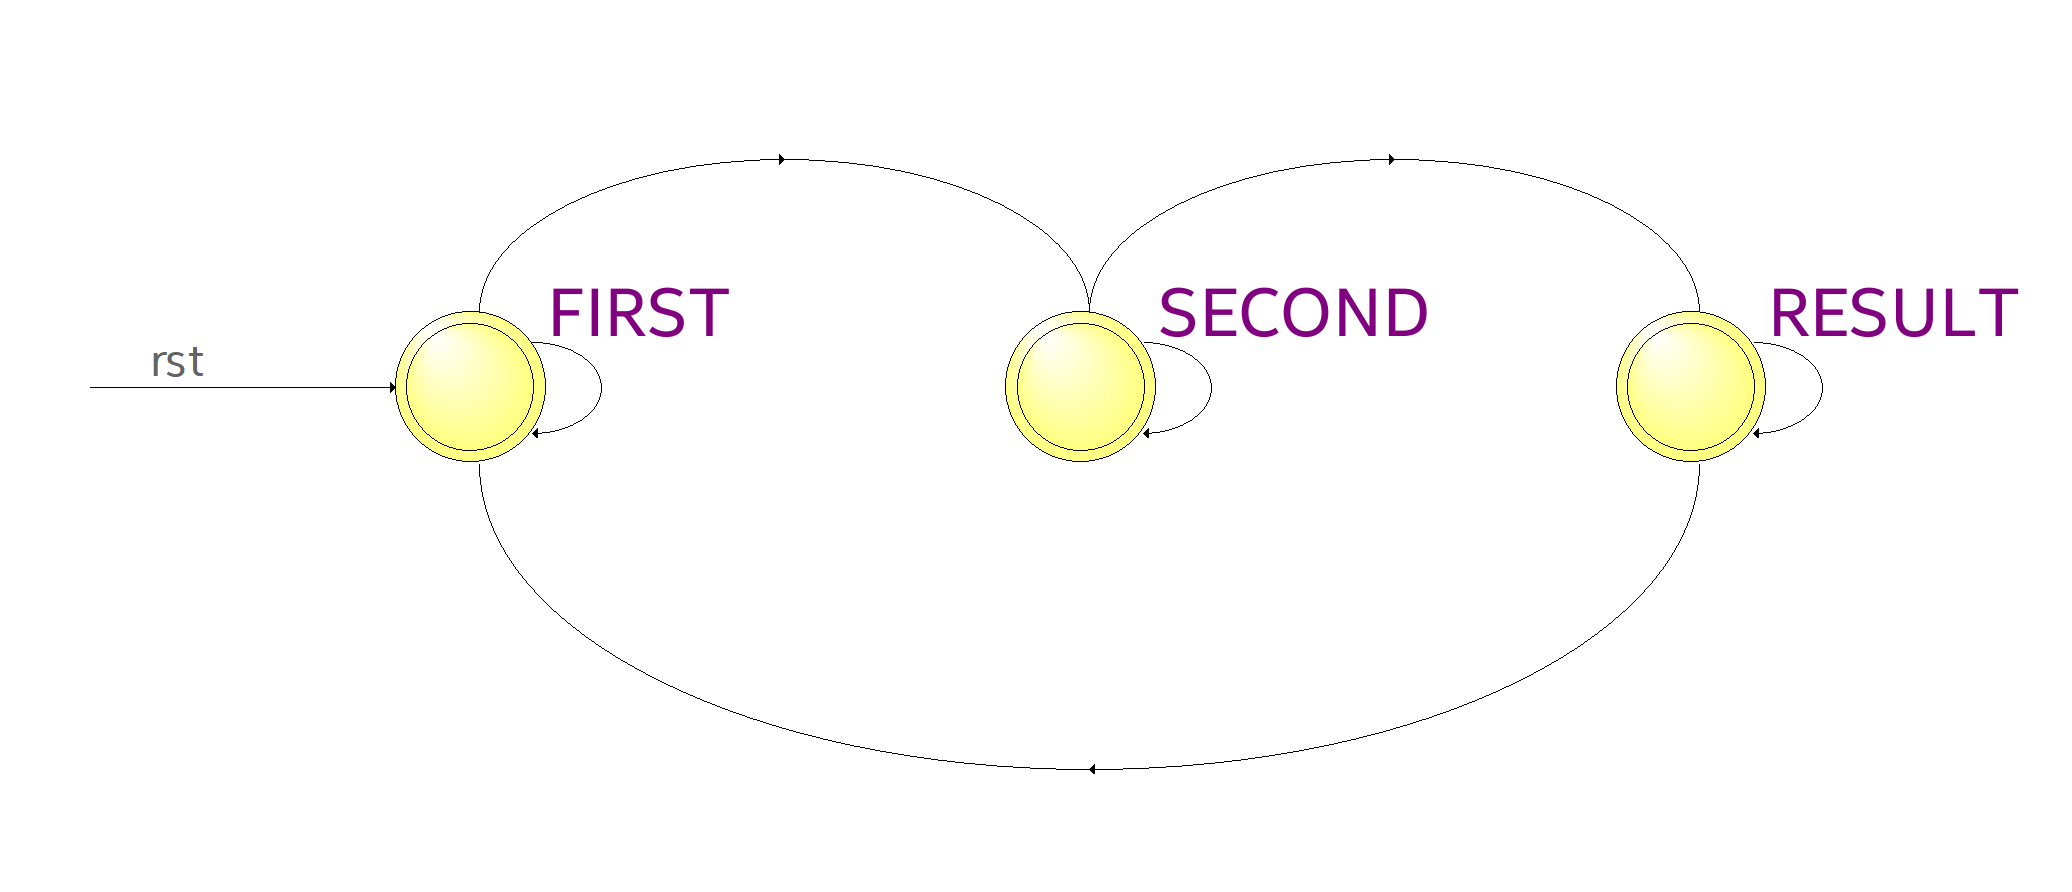
\includegraphics[width=0.8\textwidth]{mealy.png}
    \caption{mealy状态机}
    \label{fig:mealy}
\end{figure}
\subsection{顶层模块设计}
顶层模块的代码如下:
\begin{framed}
    \begin{lstlisting}[style=verilogStyle]
`include "uart_receive.v"
`include "uart_calculator.v"
`include "uart3_fre_div.v"
`include "uart_digit.v"
module uart_calculator_top(
    input clk,
    input rst,
    input rx,
    output [7:0] seg,
    output [3:0] digit
);

wire [7:0] data;
wire ready;
uart_receive uut1(
    .clk(clk),
    .rst(rst),
    .rx(rx),
    .data(data),
    .ready(ready)
);

wire [15:0] display_data;
uart_calculator uut2(
    .clk(clk),
    .rst(rst),
    .ready(ready),
    .rx_data(data),
    .display_data(display_data)
);

wire clk_div;
uart3_fre_div uut3(
    .clk(clk),
    .rst(rst),
    .clk_div(clk_div)
);

uart_digit uut4(
    .clk(clk_div),
    .rst(rst),
    .data(display_data),
    .digit(digit),
    .seg(seg)
);
endmodule
\end{lstlisting}
\end{framed}
RTL图如图\ref{fig:rtl2}所示。
\begin{figure}[!ht]
    \centering
    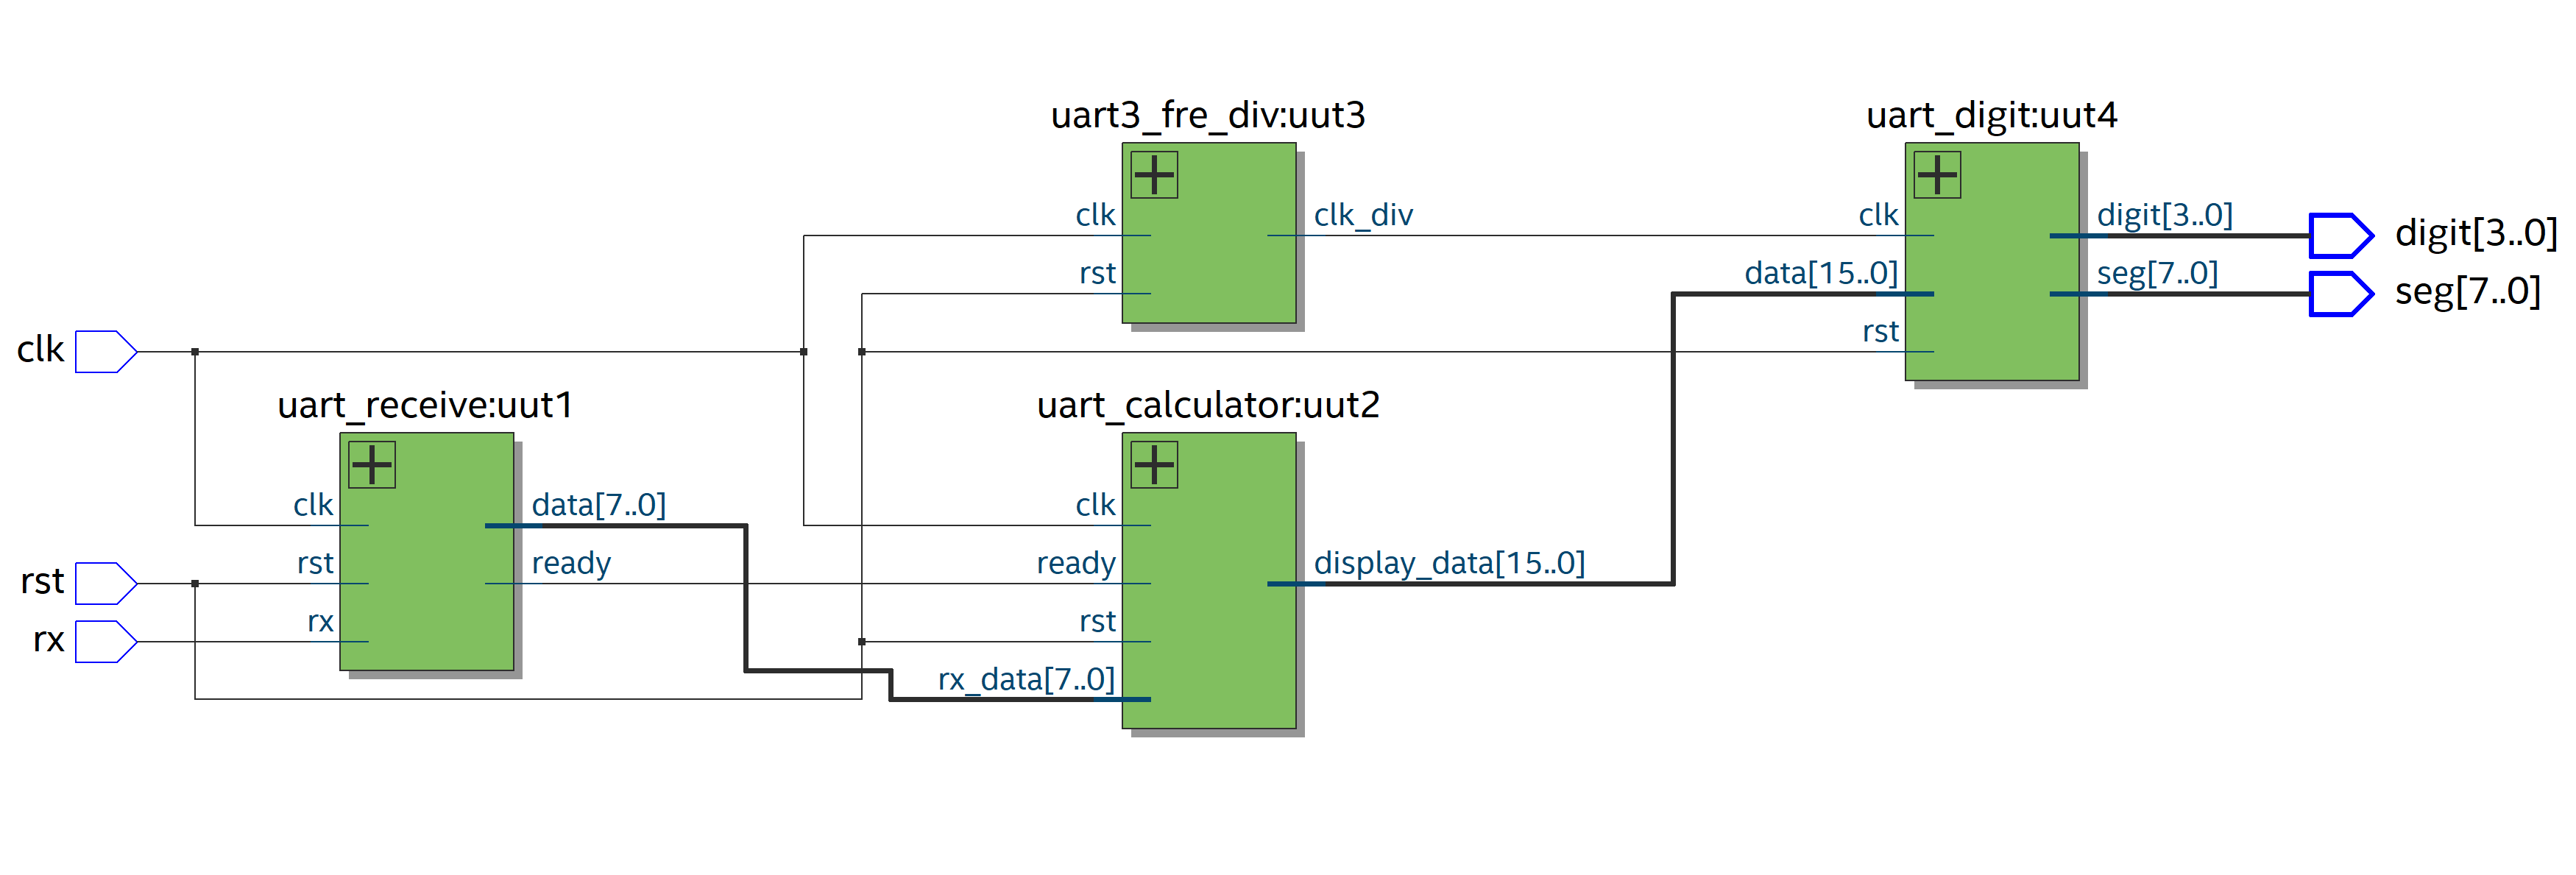
\includegraphics[width=0.8\textwidth]{rtl2.png}
    \caption{RTL图}
    \label{fig:rtl2}
\end{figure}


\end{document}